\documentclass[12pt]{beamer}
\usetheme{Pittsburgh}
\usecolortheme{seagull}
\usepackage[utf8]{inputenc}
\usepackage[english]{babel}
\usepackage{amsmath}
\usepackage{amsfonts}
\usepackage{amssymb}
\usepackage{graphicx}
\author{Design and Verification of Security Protocols and Security Ceremonies}
\title{\vspace{-.7cm}Cryptographic Primitives \\\vspace{-.7cm} Symmetric Cryptography}
%\setbeamercovered{transparent} 
\setbeamertemplate{navigation symbols}{} 
%\logo{
\includegraphics[scale=0.015]{Brasao_UFSC.png}
\includegraphics[scale=0.2]{brasao_PPGCC.jpg}} 
\institute{Programa de Pós-Graduacão em Ciências da Computacão \\ Dr. Jean Everson Martina} 
\date{\vspace{-1cm}August-November 2016} 
\subject{} 
\usebackgroundtemplate{
\includegraphics[width=\paperwidth,
height=\paperheight]{../reusable_images/fundo_UFSC.png}}
\begin{document}

{
\usebackgroundtemplate{
\includegraphics[width=\paperwidth,
height=\paperheight]{../reusable_images/fundo_capa.png}}
\begin{frame}
\titlepage

\includegraphics[scale=0.3]{../reusable_images/brasao_PPGCC.jpg}
\end{frame}
}

\begin{frame}{Cryptography Aims}
\begin{columns}
\column{.5\textwidth}
\begin{itemize}
\item To provide confidentiality;\pause
\item Securely exchange information in an insecure environment;\pause
\item Only valid users know how to perform decryption.\pause
\end{itemize}
\column{.5\textwidth}
\begin{center}
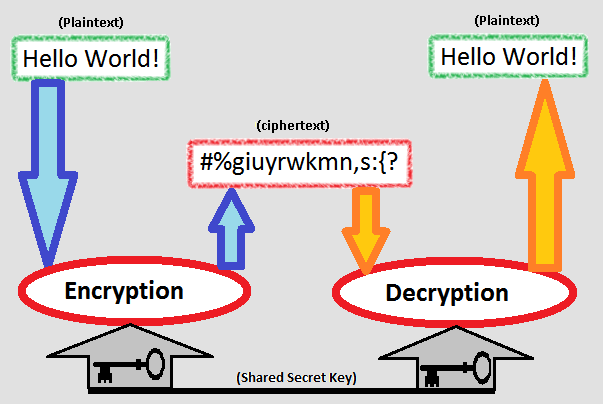
\includegraphics[scale=.35]{crypto.png}
\end{center}
\end{columns}
\end{frame}


\begin{frame}{Symmetric Cryptography Setting}
\begin{itemize}
\item Encryption and Decryption are specified algorithms;\pause
\item Two approaches:\pause
\begin{itemize}
\item Keep encryption and decryption algorithms secret: \textit{''security through
obscurity"};\pause
\item Add another variable, called a \textit{key} that must be known to encrypt and
decrypt a message;\pause
\end{itemize}
\item Symmetric-key cryptography uses same key used for both encryption and decryption.
\end{itemize}
\end{frame}


\begin{frame}{Symmetric Cryptography Problem}
\begin{itemize}
\item Symmetric-key cryptography requires that the recipient of an encrypted message knows the key;\pause
\item We can not send key in a separate message because:\pause
\begin{itemize}
\item If unencrypted an adversary could intercept it and learn the key;\pause
\item If encrypted it would require a key that had to be distributed somehow;\pause
\end{itemize} 
\item We usually assume the key is known;\pause
\item We will talk about key distribution protocols in the next lectures.
\end{itemize}
\end{frame}

\begin{frame}{Classical Cryptography}
\begin{itemize}
\item As remote as Julius Ceasar in ancient Rome or Sparta in ancient Greece;\pause
\item Substitution cipher: replace individual characters with different characters;\pause
\item Permutation cipher: change the order of the characters using permutations;\pause
\item Good modern symmetric ciphers use substitution and permutation;\pause
\item Its been the study of military schools for a long time;\pause
\item Developed the area of Cryptanalysis.
\end{itemize}
\end{frame}

\begin{frame}{Mono-alphabetic Ciphers}
\begin{itemize}
\item Same encryption algorithm used for each character;\pause
\item Problems are that:\pause
\begin{itemize}
\item Characters and words do not enough entropy;\pause
\item Context defines how characters are used and when they are used;\pause
\end{itemize}
\item You attack such ciphers by measuring the distribution on cipher-text and comparing it with a target language;\pause
\item It can be made more efficient by using context of doubles and triples.
\end{itemize}
\end{frame}

\begin{frame}{Poly-alphabetic  Ciphers}
\begin{itemize}
\item Change the substitution pattern on a character-by-character basis;\pause
\item Uses a key to configure the selection of various mono-alphabetic ciphers;\pause
\item We can not apply frequency analysis directly because the translations scheme changes every new character we input;\pause
\item You attack if the user reuses the key throughout the encryption process;\pause
\item You find the period of the key and them use frequency analysis to crack all the mono alphabetic cipher independently.
\end{itemize}
\end{frame}

\begin{frame}{Electro-Mechanical Ciphers}
\begin{itemize}
\item The enigma machine challenged the boundaries of computable functions;\pause
\item It is a machine to assist the usage of poly-alphabetic ciphers;\pause
\item Every time a key is pressed rotors turn to change the substitution pattern;\pause
\item The problems the led to Enigma being cracked are:\pause
\begin{itemize}
\item Characters never mapped to themselves;\pause
\item E() = D();\pause
\item Operator errors;\pause
\item Known plain-text;\pause
\end{itemize}
\end{itemize}
\end{frame}


\begin{frame}{Shannon's  Information Theory}
\begin{itemize}
\item In 1948, Claude Shannon invented the basis of Information Theory in his publication ``A Mathematical Theory of Communication;\pause
\item Provably secure means the key must be just as random as the cipher-text;\pause
\item This would lead to an infinite number of possible meaningful decryption;\pause
\item One-Time Pad can be implemented with Viginere or XOR;\pause
\item Provably secure if you do not reuse the key;
\end{itemize}
\end{frame}


\begin{frame}{Stream Ciphers How-To}
\begin{itemize}
\item Start with a secret key to seed a generator;\pause
\item Generate a keying stream that do not repeat itself;\pause
\item The i-th bit of keying stream is a function of the key and the first i-1 cipher-text bits;\pause
\item Combine the stream with the plain-text to produce the cipher-text (typically by XOR);\pause
\item Revert it by applying the key-stream again.
\end{itemize}
\end{frame}

\begin{frame}{Stream Ciphers Implementations}
\begin{itemize}
\item Most pre computer tools used stream ciphers;\pause
\item The German Enigma machine;\pause
\item Linear Feedback Shift Register;\pause
\item A5 – encrypting GSM handset to base station communication;\pause
\item RC-4 (Ron’s Code) WEP Encryption.
\end{itemize}
\end{frame}

\begin{frame}{Stream Ciphers Implementations}
\begin{itemize}
\item Advantages:\pause
\begin{itemize}
\item Speed of transformation: algorithms are linear in time and constant in space;\pause
\item Low error propagation: an error in encrypting one symbol Likely will not affect subsequent symbols;\pause
\end{itemize}
\item Disadvantages:\pause
\begin{itemize}
\item Low diffusion: all information of a plain-text symbol is contained in a single cipher-text symbol;\pause
\item Susceptibility to insertions/ modifications: an active interceptor who breaks the algorithm might insert spurious text that looks authentic.
\end{itemize}
\end{itemize}
\end{frame}

\begin{frame}{Block Ciphers}
\begin{itemize}
\item Encrypt a block of input to a block of output;\pause
\item Typically, the two blocks are of the same length;\pause
\item Symmetric key systems block size vary from 64 to 256 bits;\pause
\item Has different modes for encrypting plain-text longer than a block and this affects security.
\end{itemize}
\end{frame}

\begin{frame}{Block Ciphers Implementations}
\begin{itemize}
\item DES, 3-DES;\pause
\item AES;\pause
\item RC-2, RC-5;\pause
\item IDEA;\pause
\item Blowfish, Twofish;\pause
\end{itemize}
\end{frame}

\begin{frame}{Block Ciphers Implementations}
\begin{itemize}
\item Advantages:\pause
\begin{itemize}
\item High diffusion: information from one plain-text symbol is diffused into several cipher-text symbols;\pause
\item Immunity to tampering: difficult to insert symbols without detection;\pause
\end{itemize}
\item Disadvantages:\pause
\begin{itemize}
\item Slowness of encryption: an entire block must be accumulated before encryption/decryption can begin;\pause
\item Error propagation: An error in one symbol may corrupt the entire block.
\end{itemize}
\end{itemize}
\end{frame}

\begin{frame}{ECB Mode of Encryption}
\begin{columns}
\column{.5\textwidth}
\begin{itemize}
\item Simple and efficient;\pause
\item Parallel implementation possible;\pause
\item Does not conceal plain-text patterns;\pause
\item Active attacks are possible.\pause
\end{itemize}
\column{.5\textwidth}
\begin{center}
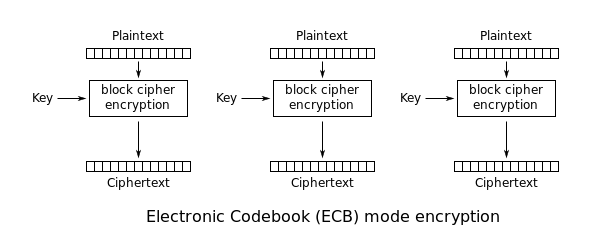
\includegraphics[scale=.25]{ECB_encryption.png}\pause\\
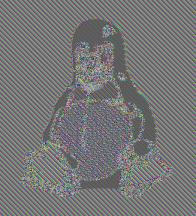
\includegraphics[scale=.35]{Tux_ecb.jpg}
\end{center}
\end{columns}
\end{frame}

\begin{frame}{CBC Mode of Encryption}
\begin{columns}
\column{.5\textwidth}
\begin{itemize}
\item It is an asynchronous stream cipher;\pause
\item Errors in one cipher-text block propagate to other blocks;\pause
\item Conceals plain-text patterns into cypher-text;\pause
\item Parallel implementation not known;\pause
\item It is difficult to manipulated Plain-text.
\end{itemize}
\column{.5\textwidth}
\begin{center}
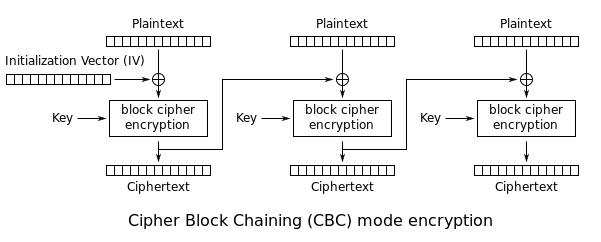
\includegraphics[scale=.25]{CBC_encryption.png}\pause\\

\includegraphics[scale=.35]{Tux_secure.jpg}
\end{center}
\end{columns}
\end{frame}

\begin{frame}{OFB Mode of Encryption}
\begin{columns}
\column{.5\textwidth}
\begin{itemize}
\item It is an asynchronous stream cipher;\pause
\item Errors in one cipher-text block propagate to other blocks;\pause
\item Pre-processing is possible;\pause
\item Conceals plain-text patterns into cypher-text;\pause
\item Parallel implementation not known;\pause
\item Active attacks are possible.\pause
\end{itemize}
\column{.5\textwidth}
\begin{center}
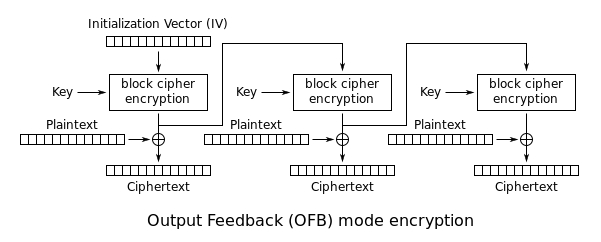
\includegraphics[scale=.25]{OFB_encryption.png}\pause\\

\includegraphics[scale=.35]{Tux_secure.jpg}
\end{center}
\end{columns}
\end{frame}

{
\usebackgroundtemplate{
\includegraphics[width=\paperwidth,
height=\paperheight]{../reusable_images/fundo_capa.png}}
\begin{frame}

{\LARGE Questions????}

\end{frame}
}

{
\usebackgroundtemplate{
\includegraphics[width=\paperwidth,
height=\paperheight]{../reusable_images/fundo_capa.png}}
\begin{frame}

\includegraphics[scale=0.8]{../reusable_images/cc_logo_arge.png}\hspace{0.5cm} 

\includegraphics[scale=0.95]{../reusable_images/by.png}

\vspace{1cm}
This work is licensed under the Creative Commons Attribution 4.0 International License. To view a copy of this license, visit http://creativecommons.org/licenses/by/4.0/.
\end{frame}
}

\end{document}